\documentclass[9pt,journal,compsoc]{IEEEtran}
\usepackage[english]{babel}
\usepackage[utf8]{inputenc}
\usepackage{cite}
\usepackage{amsthm}
\usepackage{amsmath}
\usepackage{amssymb}
\usepackage{graphicx}
\usepackage{array}
\usepackage{algorithmic}
\usepackage{url}

% correct bad hyphenation here
\hyphenation{op-tical net-works semi-conduc-tor}

\newtheorem{mydef}{Definition}


\begin{document}

\title{\huge Artificial Neural Networks in Feature Extraction: A Review}

% Author information
\author{
	\IEEEauthorblockN{Joaquim Leitão\IEEEauthorrefmark{1}}
	
	\IEEEauthorblockA{\IEEEauthorrefmark{1}jpleitao@dei.uc.pt \\ CISUC, Department of Informatics Engineering, Univesity of Coimbra, Portugal}
}

% The paper headers
\markboth{Real Time Learning in Intelligent Systems, 2016-2017}{Real Time Learning in Intelligent Systems, 2016-2017}


\IEEEtitleabstractindextext{
\begin{abstract}
	Lol, the abstract
\end{abstract}

\begin{IEEEkeywords}
	Feature Extraction, Artificial Neural Networks.
\end{IEEEkeywords}
}


% make the title area
\maketitle
\IEEEdisplaynontitleabstractindextext
\IEEEpeerreviewmaketitle


\IEEEraisesectionheading{\section{Introduction}\label{sec:introduction}}

\IEEEPARstart{I}{ntro}

Fazer intro curta

Dizer que foco na utilização de redes neuronais para efeitos de feature extraction (nao tanto de selection)

Colocar sigla para Feature Extraction - FE

4 pages

Do not forget to provide an overview of the paper!

\section{Background}\label{sec:background}

The current section addresses the importance of Feature Extraction in Intelligent Systems. In the literature this concept is often presented in the sequel of the well-known curse of dimensionality phenomenon, as a collection of methods that allow a reduction in the problem's dimensionality.

\subsection{Curse of Dimensionality}
\label{curse_dimensionality}

The curse of dimensionality refers to how certain learning algorithms may perform poorly when confronted with high-dimensional data. In many Pattern Recognition (PR) problems, low-dimension feature spaces may not allow for a good separation of the data, leading to low-accuracy classifications. By considering more features, a feature space where an hyperplane that perfectly separates the (training) data can be determined with a resulting increase in classification accuracy.

Nonetheless it has been demonstrated that, as dimensionality increases, the amount of training data needed to accurately generalise the produced classifier grows exponentially. In addition, a small \emph{training samples-to-features} ratio may also degrade performance \cite{jain2000statistical}.

A practical implication of the curse of dimensionality is that a system designer should select a small number of features when confronted with a limited training dataset. A general accepted practice is to keep the number of training samples at least ten times higher than the dimensionality: $n / d > 10$ \cite{jain2000statistical}.

\subsection{Dimensionality Reduction}

In light of the discussion conducted in \ref{curse_dimensionality}, a common interest in the vast majority of MPR applications is to keep the number of features as small as possible.

Feature Extraction and Feature Selection techniques are the most cited and recognised methods for achieving dimensionality reduction in PR problems. Feature Extraction algorithms propose a new set of features by performing transformations on a given feature set. On their turn, Feature Selection algorithms (ideally) select the best subset of features a provided feature set. As pointed out by Jain \emph{et al.} \cite{jain2000statistical}, feature extraction is typically applied before feature selection\footnote{The idea is to start by defining a new feature set based on the original one, and then select the features that, hopefully, allow a complete separation of the training data.}.

The main issues in dimensionality reduction, namely in feature extraction and selection, are related with the choice of criterion function and the appropriate dimension for the reduced feature space.

\section{Neural Networks in Feature Extraction}\label{sec:anns_feature_extraction}

Artificial Neural Networks (ANNs) have been extensively applied in the field of machine learning, in both classification and regression tasks. Because of their self-learning and trained characteristics, ANNs have also been successfully applied in FE tasks.

Considering the simplest form of ANNs, feedforward networks, FE can be obtained in the output of each hidden layer: the application of the neurons' activation function to the layer's input produces an output that can be interpreted as a set of new features \cite{jain2000statistical}. Depending on the neurons' activation function this new set of features can be a linear or nonlinear combinations of the features in the input feature set (usually is nonlinear).

In the remainder of the current section the most popular and referenced ANN architectures applied in FE tasks are intended to be covered. Such architectures include \emph{Feedforward} (namely \emph{Stacked Autoencoders}), \emph{Convolutional}, \emph{Recurrent}, \emph{Radial Basis}, \emph{Restricted Boltzmann Machines} and \emph{Self-Organising Maps}\cite{jain2000statistical, masci2011stacked, kvascev2012radial, fabius2014variational, cho2014learning, marchi2017deep}.

\textbf{FIXME: Rever a lista de arquitecturas para confirmar que não me esqueci de nehuma!!}

\subsection{Feedforward}

A feedforward ANN is one of the simplest examples of a neural network. The network is composed of several layers of neurons, where neurons in each layer are connected to neurons in the next layer: that is, connections between the units do not form a cycle. In the beginning of the current section feedforward networks were used as a motivation for the application of ANNs in FE tasks.

In its simplest forms, FE can be achieved through single or multi-layer feedforward ANNs by training the network to reconstruct the input signal in a conventional way, using a backpropagation algorithm (or other popular alternatives). This form of ANN training is considered unsupervised, as only unlabelled data is being used.

In an opposite view, a multi-layer feedforward network may be trained to perform a classification task. As multiple layers are being considered, the output of the last hidden layer (which will provide the input to the output layer) can be considered as the extracted features form the provided input sample. Networks trained with this approach have been proven to suffer from well-known \emph{vanishing gradient} problems\cite{nielsen2015neural}.

In both scenarios the FE process is learned automatically in the early layers of the final network. In recent years, namely with advances in the field of deep learning, approaches of the first type tend to be more popular and widely used.

In this sense, training of feedforward networks for FE purposes usually comprises two steps: \emph{Pre-training} and \emph{Fine tuning}.

During pre-training a series of hidden layers are trained independently in an unsupervised way: Groups of 3-layer feedforward nets (one for each hidden layer of the final network) are trained to reconstruct their respective inputs at the output layer. The idea is to make each network learn an encoder and a decoder\footnote{The encoder is learned from the input to the hidden layer, while the decoder is learned from the hidden to the output layer.}. In this process, the first network is trained with the input data; the second network is trained with the output of the first network's encoder, and so on. This process is illustrated in figure \ref{barata_saes}.

When pre-training is complete, the encoders are stacked together. Due to this last step, ANNs developed in this way are often referred to as \emph{Stacked autoencoders}.

\begin{figure}[ht]
	\centering
	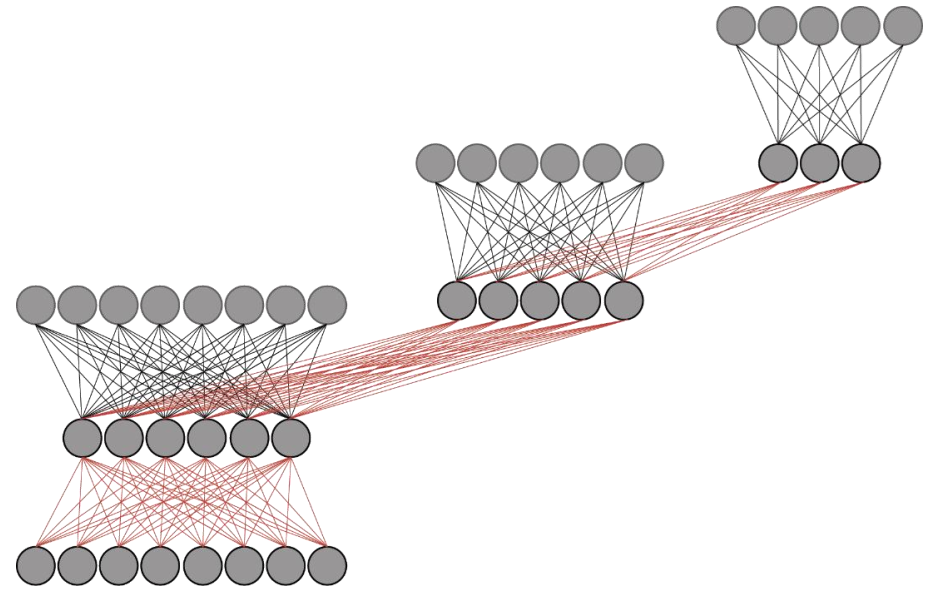
\includegraphics[scale=0.2]{stacked_autoencoders.png}
	\caption{Stacking autoencoders. Taken from \cite{barata_saes_presentation}.}
	\label{barata_saes}
\end{figure}

After the described pre-training, a fine tuning step is commonly carried out by considering an additional layer (usually with a softmax activation function) and training the network with backpropagation (or other algorithm), to lightly adjust the weights of the pre-trained layers.

At this moment it is important to address one point in the discussion: based on what has been presented, autoenconders may simply learn the identity function for both the encoder and the decoder, which is not desired. To prevent this, certain activation functions can be forced, producing \emph{regularized autoencoders} such as sparse autoencoders \cite{vincent2010stacked}, denoising autoencoders \cite{ngiam2011optimization} and contractive autoencoders \cite{rifai2011contractive}.

Feedforward networks, namely \emph{Stacked autoencoders}, can be applied for Feature Extraction purposes in a series of applications, including image processing and classification and speech recognition \cite{vincent2010stacked, lu2013speech}, just to name a few.

\subsection{Convolutional Neural Networks}

Convolutional Neural Networks (CNN) are ANNs designed to process data that comes in the form of multiple arrays, such as an image of a sequence of 1D signals. CNNs are based on four key ideas that take advantage of the properties of natural signals: local connections, shared weights, pooling and multi-layer usage \cite{lecun2015deep}. Similarly to the feedforward case, CNNs can be used to automatically extract features and perform classification tasks.

The architecture of a CNN comprises several stages: In the first few two types of layers are alternated: \emph{convolutional} and \emph{pooling} - In the literature it is common to refer to a pair of convolutional and pooling as one hidden layer of the CNN, or a \emph{slice}. Following these sequences of alternating convolutional and pooling layers, a fully connected layer is considered in order to produce the network's output. Figure \ref{convolutional_neural_net} presents a conceptual example of a CNN.

\begin{figure}[ht]
	\centering
	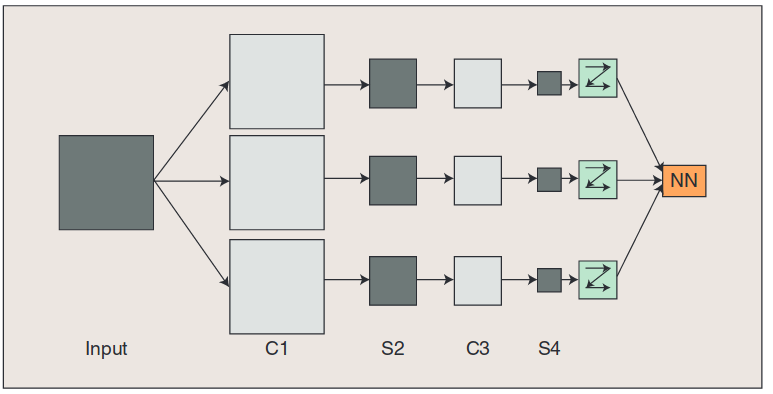
\includegraphics[scale=0.2]{Convolutional_Neural_Net.png}
	\caption{Conceptual example of a Convolutional Neural Network. Taken from \cite{arel2010deep}.}
	\label{convolutional_neural_net}
\end{figure}

In short, units in convolutional layers are organised in feature maps, where for each map a subset of units from one hidden layer serves as input to the next hidden layer. Like in other ANN architectures, each input sample has an associated weight. The same weight vector must be applied to the neurons in a single depth slice.

The logic behind the convolutional layer is to perform, for each map in a given hidden layer, a convolution of the neurons' weights with the input volume. The result of this local weighted sum is then passed through a non-linear activation function, such as a \emph{ReLU}\footnote{Rectified Linear Unit.}.

Because of the mentioned weight sharing principle, it is common to refer to the sets of weights as a \emph{filter} or \emph{kernel} that is applied to the input. For this reason, the convolutional layer is often described as consisting in the application of several filters to the input (resulting from the different feature maps considered). It can also be said that the role of this layer is to detect local conjunctions of features \cite{lecun2015deep}.

In a different view, units in the pooling layers enforce a form of non-linear down-sampling, by seeking to merge semantically similar features into one \cite{lecun2015deep}. Several non-linear functions have been proposed to this purpose, a typical pooling function is the \emph{max pooling}, which computes the maximum of a local set of units in one (or few) feature map.

From a feature extraction and dimensionality reduction point of view, the described sequence of convolutional and pooling layers is responsible for reducing the dimensionality of the provided input set. In some scenarios a normalisation layer may be considered; however, as pointed out in \cite{cs2312017convolutional}, this practice has fallen out of favor because its contribution has been shown to be minimal.

In the vast majority of the scenarios, CNNs are applied in classification problems, and for that reason additional fully-connected layers are considered where an high-level reasoning is performed. Regarding the network's training, the application of a backpropagation gradient through a CNN is similar to regular deep networks, allowing all the weights in all the layers and filters to be trained.

Convolutional Neural Networks have been extensively applied for Feature Extraction purposes, with the most sounding applications in fields such as image \cite{lawrence1997face, krizhevsky2012imagenet}, video \cite{karpathy2014large} and speech processing and recognition \cite{lecun1995convolutional, abdel2012applying}, natural language processing \cite{hu2014convolutional} and analysis of other sequences of 1D signals. CNNs were also applied to develop an artificial intelligence for the board game Go\cite{clark2014teaching, maddison2014move}

\subsection{Recurrent Neural Networks}

\subsection{Radial Basis Functions}

\subsection{Restricted Boltzmann Machines}

\subsection{Self-Organising Maps}

In Self-Organising Maps (SOM), another type of ANN used for NLFE \cite{jain2000statistical, hira2015review}, a low-dimension discretized representation of the input space is produced. Such representation is called a map.

A SOM consists of neurons with associated weight vectors (with the same dimension as the input). The neurons are positioned in the map space, usually in a two-dimensional regular spacing in either a hexagonal or rectangular grid (instead of being organised in layers, like in feedforward ANNs).

During the training of a SOM, inputs are presented to the network and, for each, the weight vector closest to the input vector is identified. Then, the weights of all the neurons in the neighbourhood of the winner neuron (that is, the one whose weight vector was selected) are updated, so that they move towards the input vector. In this way, weight vectors of neighbouring neurons in the grid are likely to represent inputs which are close in the original feature space - a "topology-preserving" map is, thus, formed \cite{kohonen1995self, villmann1997topology}. An example of an application where SOM was used for FE can be found in \cite{lawrence1997face}, although many more are available in the literature.

\section{Conclusion}\label{sec:conclusion}

Lol, conclusion

\bibliographystyle{ieeetr}
\bibliography{bibliography.bib}

\end{document}